\documentclass[10pt]{article}
\usepackage{amssymb,amsmath,times,url,graphicx,amsthm,alltt}
%\usepackage[pdftex,urlcolor=blue,pdfpagemode=none,pdfstartview=FitH]{hyperref}
\usepackage{my_packages}
\usepackage{tikz_packages}
%% url smaller font.
\makeatletter
\def\url@leostyle{%
  \@ifundefined{selectfont}{\def\UrlFont{\sf}}{\def\UrlFont{\small\ttfamily}}}
\makeatother
\urlstyle{leo}

%\usepackage[all,import]{xy}

\renewcommand{\baselinestretch}{1.2}
\date{}

\renewcommand{\thesubsection}{\arabic{subsection}. }
\renewcommand{\thesubsubsection}{\arabic{subsection}.\arabic{subsubsection} }

\theoremstyle{definition}
\newtheorem{prob}{Problem}[section]
%\renewcommand{\theprob}{\arabic{section}.\arabic{prob}}
\renewcommand{\theprob}{\arabic{prob}}

\newenvironment{subprob}%
{\renewcommand{\theenumi}{\alph{enumi}}\renewcommand{\labelenumi}{(\theenumi)}\begin{enumerate}}%
{\end{enumerate}}%

\newenvironment{matlab}
{\begin{alltt}\small\renewcommand{\baselinestretch}{1.2}\selectfont}%
{\end{alltt}}


\begin{document}



\setcounter{page}{1}
\pagestyle{plain}
\section*{MAE3145: Homework 3}
\vspace*{-0.4cm}
\noindent{Due date: \SI{2458038.1979166665}{\julianday} }%\\%\vspace*{0.5cm}

%\begin{prob}
%Consider a spacecraft moving in a potential field specified as $U(\norm{\vec r})$. The equation of motion is given by
%\begin{align}
%\ddot{\vec r} = -\deriv{U}{\vec r}.
%\end{align}
%\begin{subprob}
%\item Show that the specific angular momentum $\vec h = \vec r \times \dot {\vec r}$ is still preserved.
%\item Show that the energy $\mathcal{E}=\frac{1}{2}\dot{\vec r}\cdot \dot{\vec r} + U(\norm{\vec r})$ is preserved.
%\end{subprob}
%\end{prob}

\begin{prob}
The relative motion of the two-body problem is described by
\begin{align}
\ddot{\vec r} = -\frac{\mu}{r^3}\vec r.
\end{align}
The specific angular momentum $\vec h$ and the eccentricity $\vec e$ are defined as follows:
\begin{align*}
\vec h = \vec r \times \vec v,\quad \vec e = \frac{\vec v\times\vec h}{\mu}- \frac{\vec r}{r}.
\end{align*}
In class, we found that $\vec h$ is fixed, i.e. $\dot{\vec h}=0$. Here, we wish to show $\vec e$ is fixed according to the following steps:
\begin{subprob}
\item Using (1), show that $\dfrac{d}{dt}(\vec v\times\vec h) = -\dfrac{\mu}{r^3} \vec r\times \vec h$.
\item Using the definition of $\vec h$, show that $\dfrac{1}{r^3}\vec r \times \vec h = \dfrac{\vec r \dot r - \dot{\vec r} r}{r^2}$.\\
(Hint: $\vec a\times (\vec b \times \vec c) = (\vec a \cdot \vec c)\vec b - (\vec a \cdot \vec b)\vec c$,\; $\vec r \cdot \vec r = r^2$, and $\vec r \cdot \dot{\vec r} = r\dot r$).
\item Show that $\dfrac{d}{dt}\dfrac{\vec r}{r} = -\dfrac{\vec r \dot r - \dot{\vec r} r}{r^2}$.
\item By combining the results of parts (a), (b), and (c), show that $\dfrac{d}{dt}\vec e=0$, i.e, the eccentricity vector is fixed.
\end{subprob}
\end{prob}

\begin{prob}
A satellite is on an elliptic orbit around the Earth with a perigee radius of $r_p=7000\,\mathrm{km}$ and an apogee radius of $r_a=70000\,\mathrm{km}$. Assume that the gravitational parameter and the radius of the Earth are found on the constants sheet. Determine the following parameters (specify units in $\mathrm{km},\,\mathrm{sec},\,\mathrm{degree}$). 
\begin{subprob}
\item eccentricity $e$
\item period $T$ 
\item specific energy $\mathcal{E}$
\item true anomaly $\theta$ at which the altitude is $1000\,\mathrm{km}$.
\item velocity $v_r,v_\theta$ at the point found in part (d).
\end{subprob}
\end{prob}

%\begin{prob}
%Consider an elliptic orbit with the distance to the periapsis $r_p$ and the distance to the apoapsis $r_a$. Using the properties summarized at the third page, show that the velocity at the periapsis and the velocity at the apoapsis are given by
%\begin{align*}
%v_p = \sqrt{\frac{2\mu}{r_a+r_p}\frac{r_a}{r_p}}
%,\quad
%v_a = \sqrt{\frac{2\mu}{r_a+r_p}\frac{r_p}{r_a}}.
%\end{align*}
%
%\end{prob}

\clearpage\newpage
\begin{prob}
The specific energy and angular momentum of several asteroids heading toward the Earth have been measured as follows:

\begin{center}
\begin{tabular}{c|c|c}\hline
Asteroid & $\mathcal{E}$ $(\mathrm{km^2/s^2})$ & $h$ $(\mathrm{km^2/s})$\\ \hline
1 & $1$ & $1\times 10^5$\\
2 & $100$ & $1\times 10^5$\\
3 & $0$ & $7\times 10^4$\\
4 & $0$ & $8\times 10^4$\\
5 & $10$ & $8\times 10^4$\\\hline
\end{tabular}
\end{center}
%
We wish to determine whether any asteroid is likely to hit the Earth. The trajectory of an asteroid is assumed to be the solution of the two-body problem of the asteroid and the Earth, where \( \mu_\oplus \) is taken from the course constants sheet.

\begin{subprob}
\item Using the fact that $\mathcal{E}$ and $h$ are conserved, show that the distance at the periapsis $r_p$ satisfies the following quadratic equation:
\begin{gather}
2\mathcal{E}\, r_p^2 + 2\mu_E\, r_p -h^2=0. 
\end{gather}
(Hint: at the periapsis, $h=rv$ since $\vec r$ is perpendicular to $\vec v$.)
\item Calculate $r_p$ for all asteroids, and determine which asteroid will hit the surface of the Earth: an asteroid will hit the Earth if $r_p < R_\oplus = \SI{6378.137}{\kilo\meter}$.\\
    (Hint: In Python/\texttt{numpy}, the quadratic equation $ax^2+bx+c=0$ can be solved by the command \texttt{np.roots([a, b, c])}.)
\item For each asteroid that hits the surface of the Earth, calculate its impact velocity at the surface of the Earth.\\
(Note: the impact velocity is not same as the velocity at the periapsis.)
\item For each asteroid that does not hit the surface of the Earth, calculate its velocity when it is closest to the Earth.
\end{subprob}
\end{prob}

\begin{prob}
    Consider the point of intersection of an elliptical orbit with the \underline{semi-minor} axis.
    \begin{subprob}
    \item Prove that the following relationships are true:
        \begin{align*}
            r &= a \\
            v &= \sqrt{\frac{\mu}{r}} \\
            \theta &= \arccos \parenth{-e} 
        \end{align*}
        Hint: The first thing to try is to draw a picture. 
        Next utilize the equation of a conic section to investigate the relationships.
    \item Given the conic equation
        \begin{align*}
            r = \frac{p}{1 + e \cos \theta}
        \end{align*}
        find the derivative \(  \dot{r} \).
    \item Prove that \( \dot{r} \) possesses a maximum magnitude at the ends of the semi-latus rectum. 
    \item Show that this maximum magnitude corresponds to \( \pm e \sqrt{\frac{\mu}{p}} \).
    \end{subprob}
\end{prob}

\clearpage\newpage
\begin{prob}
    At approximately \SI{2458011.99706}{\julianday}, Cassini orbiter completed its mission studying the Saturnian system and re-entered Saturn to avoid contamination of any possible exterrestrial life in the Saturn system.
    Over the course of its nearly \SI{20}{\year} mission, Cassini studied the planet Saturn, its ring system, and numerous natural satellites. 
    In order to reach Saturn, Cassini used several gravity assist manuevers of Venus, Earth and Jupiter, in order to increase its orbital velocity with respect to the Sun and gain enough energy to intercept Saturn. 
    The Cassini mission remains the largest interplanetary vehicle launched by the United States, consisting of the Cassini Orbiter and Huygens lander.
    The Huygens lander parachuted to a soft landing on Titan on \SI{2458011.99706}{\julianday} and remains the most distant interplanetary landing of any human-made vehicle.
    \begin{figure}[htbp]
        \centering
        \subcaptionbox{Cassini Interplanetary Trajectory\label{fig:cassini_interplanetary}}{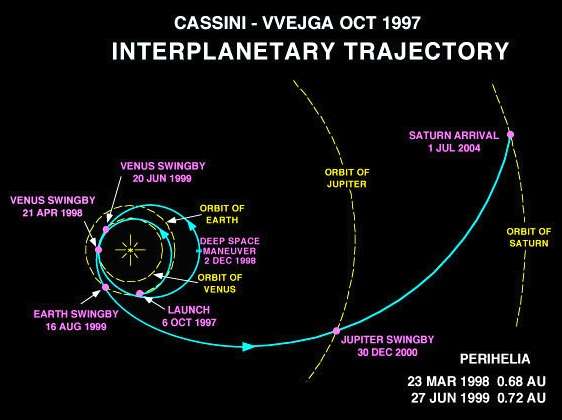
\includegraphics[width=0.5\textwidth]{figures/cassini_trajectory.jpg}}~
        \subcaptionbox{Cassini Trajectory 2004 to 2005\label{fig:cassini_traj}}{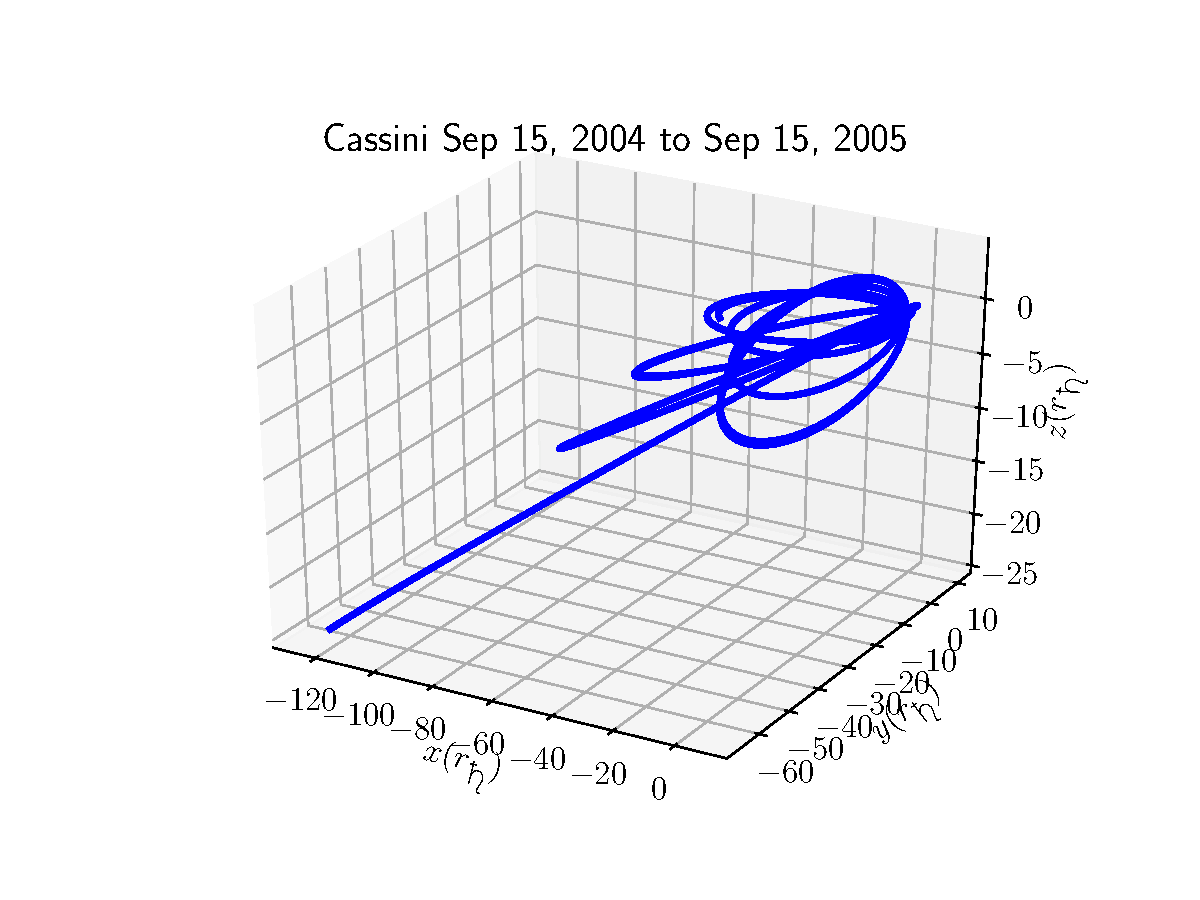
\includegraphics[width=0.5\textwidth]{figures/Figure_1.pdf}}\\
       \subcaptionbox{Cassini Orbiter\label{fig:cassini_orbiter}}{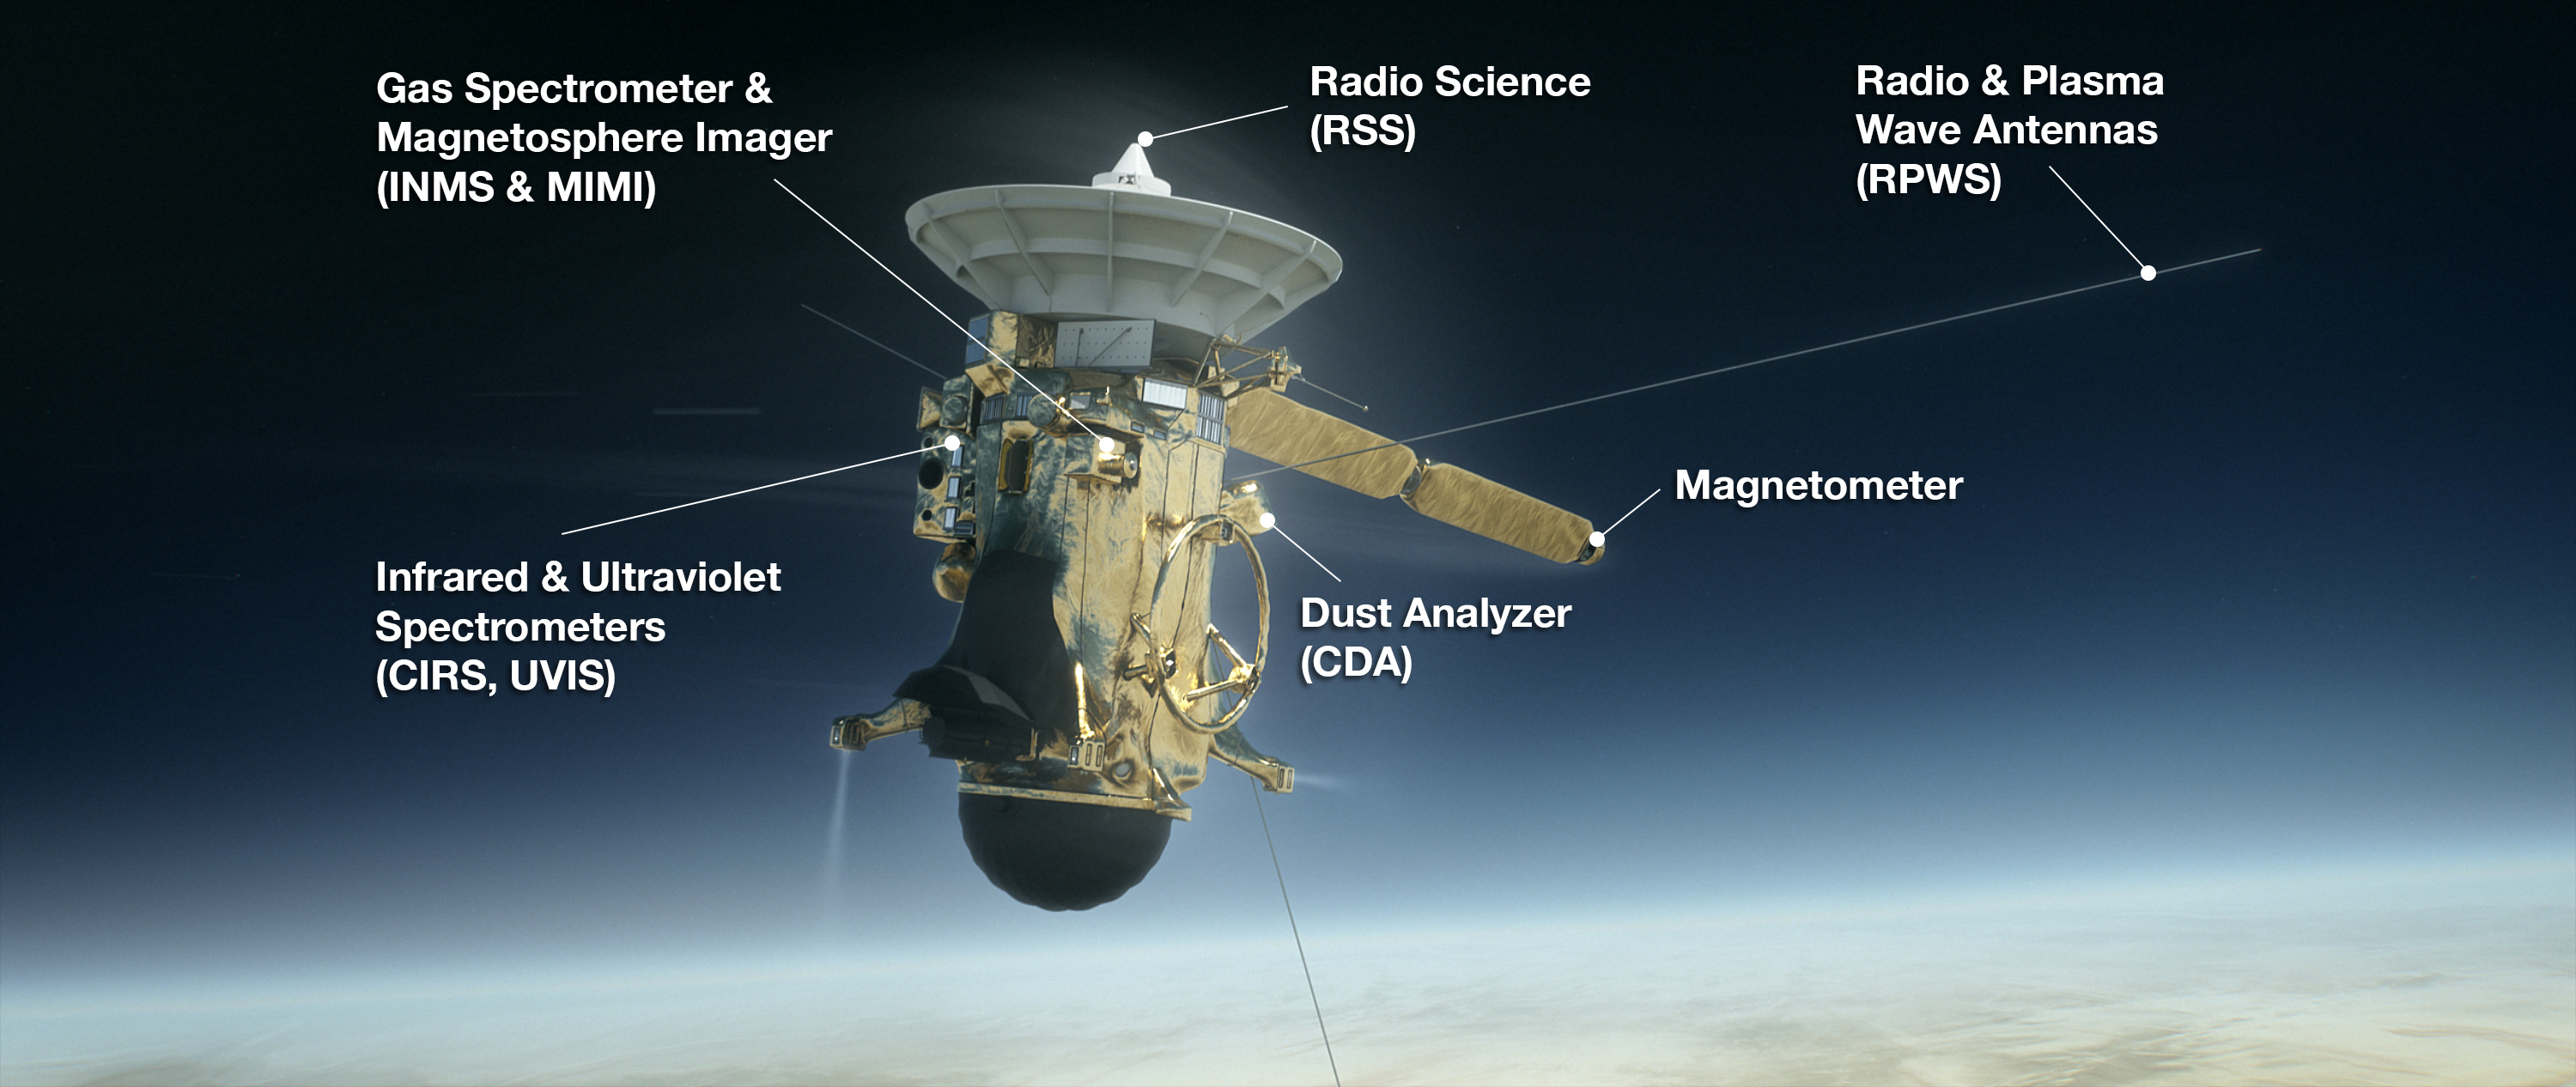
\includegraphics[width=0.8\textwidth]{figures/7754_CassiniPlungeInstrumentsLabeled.jpg}}
       \caption{Cassini Mission} 
    \end{figure}

    Here we will investigate the orbit of Cassini 13 years ago on Sep 15, 2004.
    On this date, the position and velocity of Cassini with respect to Saturn barycenter are given as 
    \begin{align*}
    \bar{r} &= \begin{bmatrix} -7546026.6144396 & -3717105.21901527 & -1515557.34280287\end{bmatrix} \si{\kilo\meter} \\
    \bar{v} &= \begin{bmatrix}  0.89506649 & -0.33312074  & 0.21519571 \end{bmatrix} \si{\kilo\meter\per\second}
    \end{align*}

    \begin{subprob}
        \item Given this position and velocity vector, determine the type of orbit of Cassini.
        \item Determine the period \( P \), angular momentum vector \( \bar h \), semi-latus rectum \( p \), specific mechanical energy \( \mathcal{E}\), eccentricity \( e \), true anomoly \( \nu \), and radius of periapsis and apoapsis \( r_p, r_a\).
        \item How does the velocity of Cassini compare to the velocity of a circular orbit at this radius, i.e. compare \( v \) and \( \sqrt{2} v_c \)?
            Should the velocity of Cassini be less than or greater than \( \sqrt{2} v_c \)? Why or why not?
        \item Using Python, create a diagram of the orbital plane and the location of Cassini.
            Mark the location of periapsis and the local horizontal/local vertical unit reference frame, \( \hat r, \hat \theta \) as well as the perifocal reference frame \( \hat p, \hat q \).
        \item The major subdivisions of the Saturn ring system are copied below from \href{https://en.wikipedia.org/wiki/Rings_of_Saturn#Major_subdivisions}{Wikipedia}.
            Based on the current orbital properties, which ring subdivision does Cassini pass through.
            \begin{figure}[htbp]
                \centering
                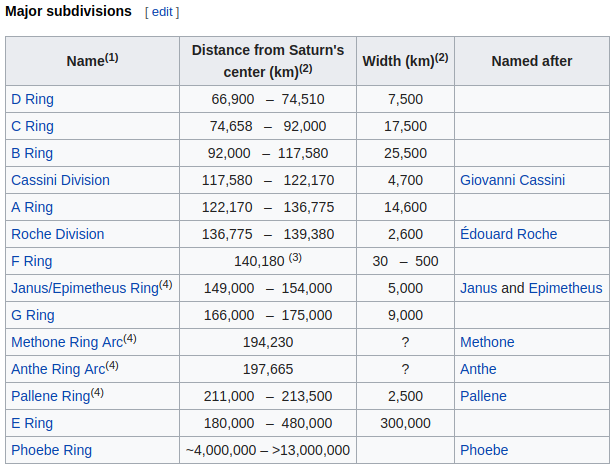
\includegraphics[width=0.5\textwidth]{figures/ring_subdivisions.png}
                \caption{Ring Subdivisions}
            \end{figure}
    \end{subprob}
\end{prob}

\begin{prob}
    In a chance meeting in the Science and Engineering hall, you've bumped into Elon Musk.
    He is the CEO of Tesla Motors and SpaceX and is planning on sending manned missions to Mars.
    Unfortunately, Mr.~Musk has never taken an astrodynamics class and is in need of your help to plan his latest mission.
    \begin{subprob}
    \item The Dragon capsule is in a circular parking orbit of the Earth, at an altitude of \SI{120}{\kilo\meter}.
    To begin a voyage to Mars, what velocity does the satellite require to \underline{escape the Earth}.
    \item Would your answer be different for an elliptical orbit ( \( e = 0.3\), \( \nu = \SI{145}{\degree} \), with \( a \) the same as the previous problem)?
        Why or why not?
    \item If you assume both burns are tangent to the existing velocity, what are the required increases in velocity for each of the previous cases?
    \end{subprob}
\end{prob}

\clearpage\newpage
\begin{prob}
    The data below are composed of postion, \( \bar r \) in \si{\kilo\meter}, and velocity, \( \bar v \) in \si{\kilo\meter\per\second} vectors in the local vertical/local horizontal frame. 
    Each row corresponds to the state of a particular satellite in Earth orbit. 
    The first three columns define the position vector \( \bar r = r_1 \hat r + r_2 \hat \theta + r_3 \hat h \; \si{\kilo\meter} \) and the last three columns define the velocity vector \( \bar v = v_1 \hat r + v_2 \hat \theta + v_3 \hat h \; \si{\kilo\meter\per\second} \).

    \begin{verbatim}
6781.675224   0.000000   0.000000  -0.002574   7.667057   0.000000
41655.940637   0.000000   0.000000  -1.103624   1.706184   0.000000
6894.474715   0.000000   0.000000  -0.184823   8.038042   0.000000
7491.578823   0.000000   0.000000  -0.859794   7.408067   0.000000
35855.749929   0.000000   0.000000  -1.479844   1.890930   0.000000
38208.441964   0.000000   0.000000  -0.925821   2.167744   0.000000
    \end{verbatim}
For example, the first row of this data set corresponds to the position and velocity of the International Space Station,
\begin{align*}
    \bar r &= 6781.675224 \, \hat r + 0 \, \hat \theta + 0 \, \hat h \, \si{\kilo\meter}, \\
    \bar v &= -0.002574 \, \hat r + 7.667057 \, \hat \theta + 0 \, \hat h \, \si{\kilo\meter\per\second\squared}.
\end{align*}
    For the given orbital data determine the following for each satellite.
    Units should be provided in seconds, degrees, and kilometers.

    \begin{subprob}
    \item Orbital properties
    \begin{itemize}
        \item Period -- \( P \) 
        \item Specifc mechanical energy -- \( \mathcal{E} \) 
        \item Semi-major axis, semi-latus rectum, eccentricity, true anomaly
        \item Radius of periapsis and apoapsis -- \( r_p, r_a \)
        \item Angular momentum vector and magnitude -- \( \bar h \)
        \item Flight path angle -- \( \gamma \)
        \item Position and Velocity vectors in the perifocal reference frame
    \end{itemize}

    The orbital properties of the first satellite (first row) is given below.
    You should provide your hand calculations demonstrating the computation of the orbital properties for this case. 
    This test case is used to verify your software is working correctly.
    For the other cases, you can simply provide the output of your program.
\item Using Python, plot the orbit of each satellite in the perifocal reference frame and mark the location of the satellite.
    Mark the location of periapsis and apoapsis on your plot as well as the local horizontal/local vertical frame, and flight path angle.
    Some of these satellites are in nearly circular orbits so the difference between periapsis and apoapsis will be difficult to notice in your plots.
    \end{subprob}

Solution for first satellite:

\clearpage\newpage
    \begin{verbatim}
0 ISS (ZARYA) 25544                                                                                                                                                                           
Satellite State                                                                                                                                                                               
Position and Velocity in LVLH frame                                                                                                                                                           
r_hat:          6781.6752240256 km rd_hat:    -0.00257359868086831 km/sec                                                                                      
t_hat:                        0 km td_hat:        7.66705746939915 km/sec                                                                                                                     
h_hat:                        0 km hd_hat:                       0 km/sec                                                                                                                     
                                                                                                                                                                                              
Position and Velocity in EPH/PQW frame                                                                                                                                                        
e_hat:         2453.84042760766 km ed_hat:        7.14662603444703 km/sec                                                                                                                     
p_hat:        -6322.16624267355 km pd_hat:        2.77660101315318 km/sec      
h_hat:                        0 km hd_hat:                       0 km/sec      
                                                                               
Position and Velocity in IJK frame                                             
i_hat:        -4226.54578373763 km id_hat:       -1.66958104755974 km/sec      
j_hat:         3746.04288415422 km jd_hat:       -6.15442824782474 km/sec      
k_hat:        -3754.27653379581 km kd_hat:       -4.25667580753874 km/sec      
                                                                               
RAD_MAG   :      6781.6752240256 km = 4.53326990820498e-05 AU                  
VEL_MAG   :     7.66705790133865 km/sec                                        
                                                                               
Orbital Elements                                                               
sma:           6782.55976540987 km raan:          286.709516148979 deg         
ecc:       0.000360113803137797    arg_p:         293.694918634304 deg         
inc:                     51.643 deg nu:            291.21286881209 deg         
                                                                               
Elliptic Orbital Parameters                                                    
P         :     6782.55888583428 km = 4.53386059964241e-05 AU                  
ANG MOM   :     51995.4936814046 km^2/sec                                      
PERIOD    :     5559.06039988679 sec =       1.544183444413 hr                 
ENGERGY   :    -29.3842231979148 km^2/sec^2
RAD_PER   :     6780.11727201773 km = 4.53222848160721e-05 AU
RAD_APO   :       6785.002258802 km = 4.53549389359755e-05 AU

VEL_CIRC  :     7.66655800402987 km/sec
VEL_ESC   :     10.8421503060191 km/sec
TRUE_ANOM :      291.21286881209 deg
FPA       :  -0.0192324549052291 deg
ECC_ANOM  :     291.232102521087 deg
MEAN_ANOM :     291.251334975467 deg
MEAN_MOT  :    0.064759145269825 deg/sec

T_PAST_PER:     4497.45489632301 sec =     1.24929302675639 hr
    \end{verbatim}
\clearpage\newpage
NOTE: You will need to add some additional information to your plot. 
This can be done by hand or within Python.
The plot shown below is \textbf{NOT COMPLETE} but is only here for illustration purposes.

\begin{figure}[htbp]
    \centering
    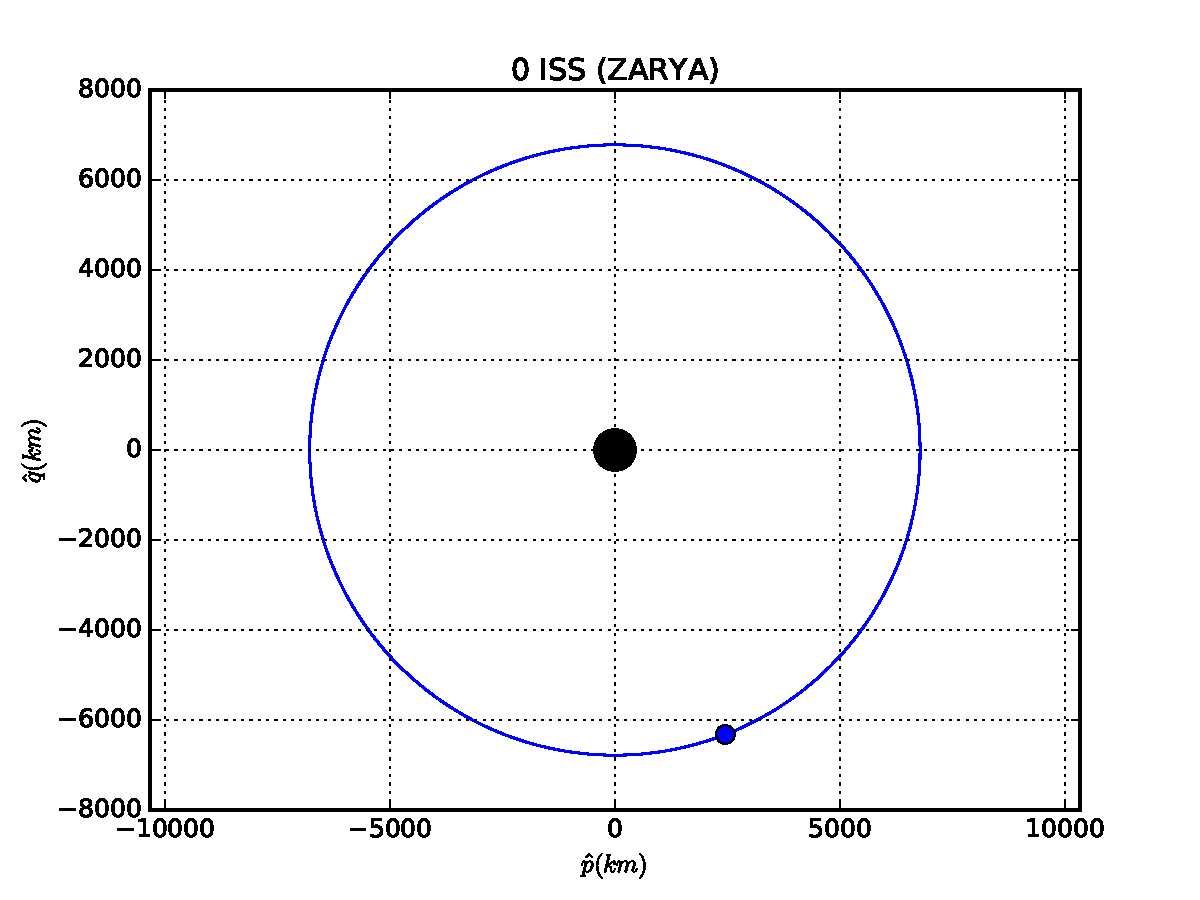
\includegraphics[width=\textwidth]{figures/25544.pdf}
    \caption{First satellite orbital plane plot\label{fig:iss}}
\end{figure}
\end{prob}
\end{document}


